


Distributed computing deals with the execution of code on multiple computers
connected to a network. As stated in \cite{andrewsfoundations}: "\emph{Distributed
computing is a field of computer science that studies distributed systems. A
distributed system consists of multiple autonomous computers that communicate
through a computer network. The computers interact with each other in order to
achieve a common goal. A computer program that runs in a distributed system is
called a distributed program, and distributed programming is the process of
writing such programs.}"

\begin{figure}[htb]
    \centering
    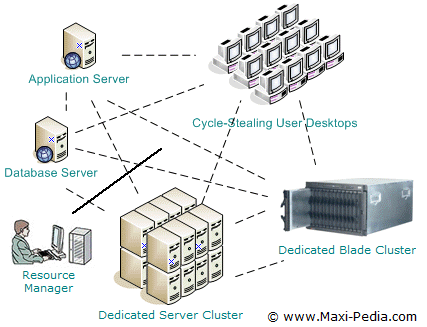
\includegraphics[width=\columnwidth]{DistributedComputing}
    \caption{General structure of a distributed computing system.}
    \label{fig:distributed-computing}
\end{figure}

The term refers to a wide range of different application (i.e. grid computing,
cloud computing, \nameref{sec:bg:crowd:auto:parasitic}, jungle computing
\footnote{Winner of the coolest name 2012}) so there is a need of a further
categorization of 


% cos'è automatic omputation
%% grid computing dove vengono eseguiti task
%% 
Unlike human computation, \emph{automatic computation} aim at executing task, or
part of it, in an automatic fashoin, without user interaction. This kind of
\emph{distributed computation} leverage on the existence of a \emph{grid} of
connected nodes able to perform data intensive calculation.

The platforms that implement these solution use different frameworks for splitting
algorithms into atomic operation executable by the nodes. One of these frameworks
is MapReduce\footcite{dean2008mapreduce} that, using the core concept of
\emph{Divide et impera} can produce highly parallelizable algorithms.\\

\emph{Automatic computation} cen be further subdivided accordingly to the will
of the user to perform computation on its computer.

\subsubsection{Voluntary computing}
\label{sec:bg:crowd:auto:voluntary}
% spiego boinc/SETI funzionamento

%% TODO ??? rifa
When a user want to share the computational power of its computer to some
project he/she think are worth of it, then might think of using the \ac{BOINC}
system.\\

\begin{figure}[htb]
    \centering
    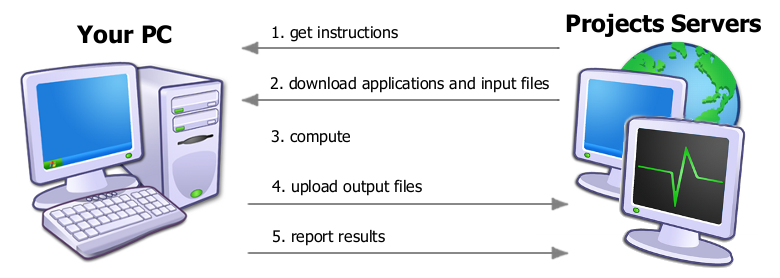
\includegraphics[width=0.5\columnwidth]{boinc}
    \caption{The \acs{BOINC} logo.}
    \label{fig:boinc}
\end{figure}
The \ac{BOINC} system was originally developed to support the \ac{SETI@home}
project, before it became used as a platform for other distributed computing
applications. \ac{BOINC} is an open source middleware system for volunteer
and grid computing. It consist on two parts, the backend server, running on
linux pletfomrs, and the client, cross-platform, for the end-user.\\

This piece of software allow a user to connect to the \ac{BOINC} grid, by doing
so a user is allowing the \ac{BOINC} client to use the idle time of its CPU to
perform computation. The client can now  download all the necessary data from the
chosen project site alonside with the code to run, once all the downloads are
completed the \ac{BOINC} client can run the code and send the results back to
the project site.\\

There are over 40\footnote{At the time of writing.} projects that leverage on
the \ac{BOINC} platform to perform computation on different application areas,
for example the aforementioned \ac{SETI@home} project use this framework to
search for extraterrestrial intelligence by analyzing the narrow-band radio
signal coming from the Arecibo radio telescope.


\subsubsection{Parasitic computing}
\label{sec:bg:crowd:auto:parasitic}
% Spiego l'idea
% chi è stato
% e perchè
% come funziona

Parasitic computing\footnote{In this thesis we are not covering, neither
we are interested in, the ethical or moral implication of using this technique.}
is a technique that, using some exploits and ad-hoc code, allow a \emph{malicious}
user to use the computational power of the \emph{victim} computer without this
being aware. As one can notice parassitic compiting has a strong relationship
with \emph{distributed computing}, in fact is a specialization of the general
class of \emph{voluntary computing}, where the user is unaware of
the execution\footnote{In \emph{voluntary computing} the user can be unaware
of the actual code they are executing, but they are aware of the execution.}.\\

This approach was first proposed by \cite{barabasi2001parasitic} to solve the
NP-complete 3-SAT problem using the existing TCP/IP protocol stack and its error
handling routines. The satisfiability problems or "SAT" involves finding a
solution to a boolean equation that satisfies a number of logical clauses. For
example, $(x_1 \oplus x_2) \land (x_2 \land x_3 )$ in principle has $2^3$ potential
solutions, but it is satisfied only by the solution: $x_1=1, x_2=0, x_3=1$.
Problems problem like the one in the example are known as 2-SAT problem because
each clause, shown in parentheses, involves two variables. The more difficult
3-SAT problem is known to be NP-complete, which in practice means that there is
no known polynomial-time algorithm which solves it.\\
\begin{figure}[htb]
    \centering
    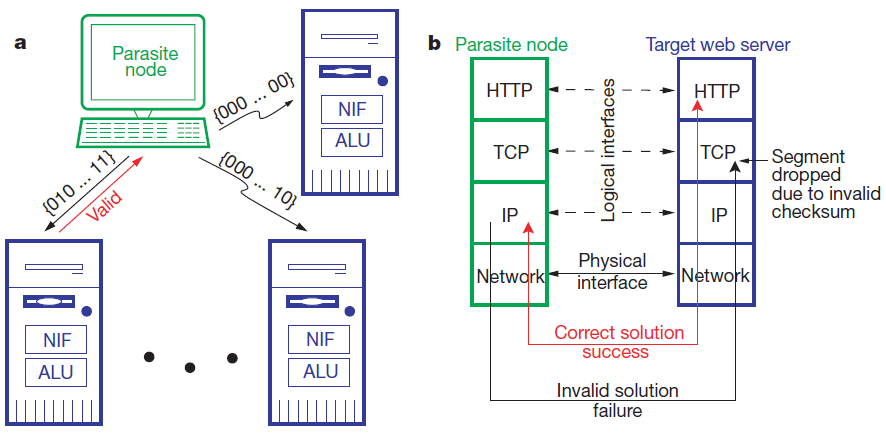
\includegraphics[width=\columnwidth]{parasitic}
    \caption{Schematic diagram of the parasitic computer solving the 3-SAT
    problem.}
    \label{fig:parasitic}
\end{figure}

The approach proposed in the paper was to perform a brute force attack to guess
the right solution of a 3-SAT problem using a parallel apprach as depicted in
\autoref{fig:parasitic}. The parasite node creates $2^n$ specially constructed
messages designed to evaluate a potential solution. These messages are sent to
many target servers throughout the Internet. After receiving the message, the
target server verifies the data integrity of the TCP segment by calculating a
TCP checksum. The construction of the message ensures that the TCP checksum fails
for all messages containing an invalid solution to the posed SAT problem. Thus,
a message that passes the TCP checksum contains a correct solution. The target
server will respond to each message it receives (even if it does not understand
the request). As a result, all messages containing invalid solutions are dropped
in the TCP layer. Only a message which encodes a valid solution \emph{reaches}
the target server, which sends a response to the \emph{request} it received.\\

This approach may seem wrong or at leat not right, with respect to the user, but
if one think about it notice how we are always making computation without even
knowing. \ac{GWAP} or application like \href{http://www.google.com/recaptcha}{reCAPTCHA}
are examples of involuntary human computation (as in \autoref{tab:matrix}). So
they are using the same technique to perform a sort of \emph{parasitic human
computing} without complainig about the user will.\\

To avoid the ethic implication of doing \emph{parasitic computing} a hybrid
approach (parasitic/voluntary) can be used. If the user give the permission to
run computation on its computer exchange of a return of any type, then we are
able to score the best on both approaches. A similar solution was proposed in
\cite{karame2011pay}.
In this paper they propose a microcomputations as micropayments in web-based
services. Their solution is to give the user access to online contents (such as
newspaper, video, etc.) after performing small \js{} computation.

\paragraph{Parasitic \js{}} described in \cite{jenkin2008parasitic} can be
considered an enhancement of the solution proposed by \cite{barabasi2001parasitic},
since using \js{} and the HTML5 features to their full potential (see
\ref{sec:bg:web:html5}) we are able to perform any kind of computation
within the browser window/tab. \js{} offers also a standard platform for the
exection of code without the need of any ad-hoc software for each platform.
Furthermore all the code executed by a browser run in a sandboxed environment,
keeping the user computer safe from any malicuis intent.